\scanpage{66}
\[
\unsure{\mathscr A|\mathcal A}\qquad \deleted{\theta^2=0}
\]
\[
A-\unsure{B|\mathscr B}
\]
\[
\theta_{\unsure{xx'|xu}}=\qquad\theta\deleted{\unsure{B}}
\]
\[
\theta^2=0\qquad\deleted{\unsure{A\theta\theta1|A\theta\theta_1}}
\]
\[
\unsure{\varphi|\phi}\qquad \pi_{x'}\theta\pi_x=\theta_{xx'}
\]
\figure{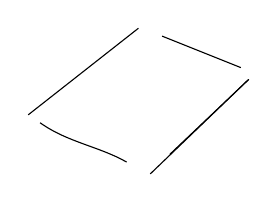
\begin{tikzpicture}
\draw (0,0)--(1.4,1.1) (1.7,1)--(2.7,.6) (2.8,.45)--(1.55,-.75) (.15,-.1)..controls(.5,-.35)and(.9,-.4)..(1.25,-.6);
\draw (2.8,.45)--(1.8,-.5);
\end{tikzpicture}}
\[
\deleted{x_1\unsure{\in|<}x_2\unsure{\in|<}x}
\qquad x_1\geq x_2\geq x_3\;\text{--}\;\geq\underbrace{x_n\geq x_{n+1}}\geq x_{\unsure{n+m|n+2}}
\]
\[
\theta_{x_1,\unsure{x_2|x_n}}\quad\theta
\]
\[
\pi_{x_{\unsure{m|n+m}}}\theta\;\text{--}\;\pi_{x_{n+2}}\theta\pi_{x_{n+1}}
\underbrace{\varphi_{x_n x_{n+1}}\pi_{x_n}}
\underbrace{\theta\cdots\pi_{x_3}\theta\pi_{x_2}\theta\pi_{x_1}}
\]
\figure{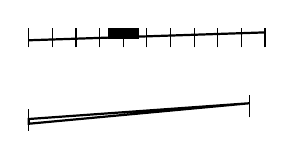
\begin{tikzpicture}
\draw[thick] (0,1)--(3,1.1);
\foreach \x in {0,.3,.6,.9,1.2,1.5,1.8,2.1,2.4,2.7,3}{\draw (\x,.91)--(\x,1.15);}
\fill (1,1.02) rectangle (1.4,1.16);
\draw[thick] (0,0)--(2.8,.2)--(0,-.06)--cycle;
\draw (0,-.15)--(0,.13) (2.8,.02)--(2.8,.3);
\end{tikzpicture}}
\[
\unsure{\varphi_n|\varphi_x}\qquad\unsure{\varphi_{x'}|\theta_{x'}}
\]
\figure{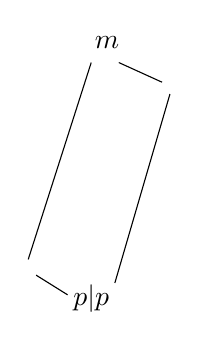
\begin{tikzpicture}
\draw (0,0)--(.8,2.5) (1.15,2.5)--(1.7,2.25) (1.8,2.1)--(1.1,-.3) (.1,-.2)--(.5,-.45);
\node at (1,2.75) {$\unsure{m}$}; \node at (.8,-.5) {$\unsure{p|\mathfrak p}$};
\end{tikzpicture}}
\[
\left\{\begin{aligned}
&\theta\quad A\text{-\unsure{linéaire}}\\
&\theta^2=0\\
&\theta\text{ de degré }1
\end{aligned}\right.
\qquad\theta
\]
\diagram{\begin{tikzcd}[ampersand replacement=\&,row sep=small,column sep=small]
\bullet \arrow[dd,bend right=30] \&\&\\
\bullet\arrow[d] \& {}\arrow[r,dash] \&\bullet\arrow[d]\\
\bullet \& {}\arrow[l] \&\bullet \&\bullet\arrow[l]\arrow[ll,bend left=35]
\end{tikzcd}}
\figure{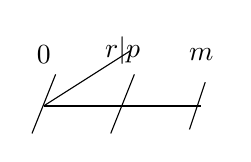
\begin{tikzpicture}
\draw[thick] (0,0)--(2,0);
\draw (-.15,-.35)--(.15,.4) (.85,-.35)--(1.15,.4) (1.85,-.3)--(2.05,.3);
\draw (0,0)--(1.1,.7); \node at (0,.65) {$0$};\node at (1,.7) {$\unsure{r|p}$};\node at (2,.65) {$\unsure{m}$};
\end{tikzpicture}}
\margin{$\operatorname{Hom}$}
\[
\unsure{\mathscr H|\mathcal H}
\]
\deleted{anneau gradué topologique,}

$\mathscr A^*$ \deleted{$\unsure{\mathscr H|\mathscr A}$} \unsure{algèbre topologique} \inserted{(\unsure{séparée, complète})} \unsure{graduée} sur $A$, à degrés $\geq0$, avec
\[
\left\{\begin{aligned}
\mathscr A_0^{\unsure{0|\circ}}&=\deleted{\unsure{\simeq}}\prod_{x\in X}\widehat{\unsure{\mathscr O|\mathcal O}}_x
\quad\text{d'où des}\quad\pi_x\in\mathscr A_0\quad(x\in\unsure{X|\mathscr X})\\
&\text{(\unsure{isom d'$A$-algèbres topologiques})}\\
\theta&\in\mathscr A_1^1,\quad\text{avec}\quad\underline{\theta^2=0},\quad
\underline{\pi_{x'}\theta\pi_x=0\quad\deleted{\unsure{x}}\quad\text{si $x'$ ne \unsure{précède} pas $x$}}
\end{aligned}\right.
\]
$\mathscr A$ libre pour ces propriétés \text{------}
% archive sheet number: 65
